\documentclass[12pt]{standalone}

\usepackage{tikz}
\usepackage{ctex}

\begin{document}
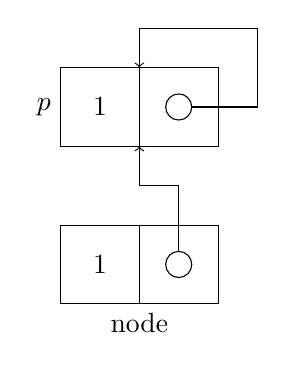
\begin{tikzpicture}

\draw (0,0) rectangle node {$1$} (1,1) 
    (1,0) rectangle node[circle,draw] (A) {} (2,1);
\draw (0,-2) rectangle node {$1$} (1,-1) 
    (1,-2) rectangle node[circle,draw] (B) {} (2,-1);

\draw[->] (A) -- ++(1,0) -- ++(0,1) -- ++(-1.5,0) -- ++(0,-0.5);
\draw[->] (B) -- ++(0,1) -- ++(-0.5,0) -- ++(0,0.5);

\node[left] at (0,0.5) {$p$};
\node[below] at (1,-2) {node};

\end{tikzpicture}
\end{document}
